\documentclass[tikz,border=2pt]{standalone}
\usepackage{amsmath,amssymb}
\usepackage{pgfplots}
\pgfplotsset{compat=1.18}

\begin{document}
% The pointwise inequality behind Markov: for a nonnegative nondecreasing f, the step
% f(a) 1{x >= a} lies below f(x) everywhere. Shown for f(x) = x and f(x) = x^2/a.
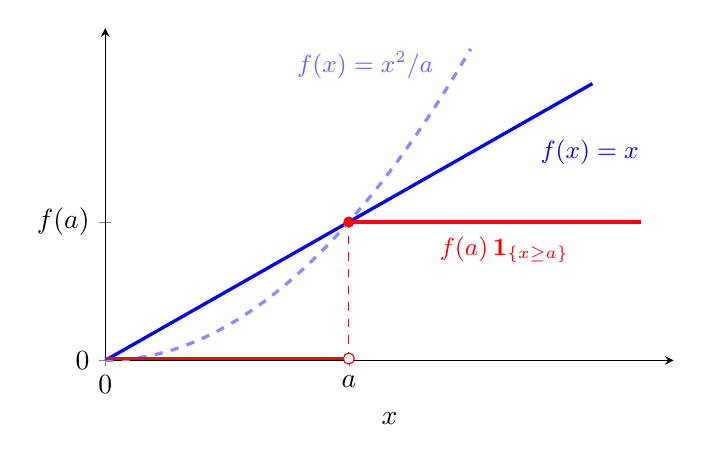
\begin{tikzpicture}
	\begin{axis}[
		axis lines=left, xmin=0, xmax=3.5, ymin=0, ymax=3.6,
		xtick={0,1.5}, xticklabels={$0$,$a$}, ytick={0,1.5}, yticklabels={$0$,$f(a)$},
		xlabel={$x$},
		samples=100, smooth, width=8.8cm, height=5.8cm, clip=false
		]
		\addplot[blue, very thick, domain=0:3.0] {x};
		\addplot[blue!45, very thick, dashed, domain=0:2.25] {x^2/1.5};
		\addplot[red, very thick] coordinates {(0,0.02) (1.5,0.02)};
		\addplot[red, very thick] coordinates {(1.5,1.5) (3.3,1.5)};
		\draw[red, dashed] (axis cs:1.5,0) -- (axis cs:1.5,1.5);
		\fill[red] (axis cs:1.5,1.5) circle (2pt);
		\draw[red, fill=white] (axis cs:1.5,0.02) circle (2pt);
		\node[blue, anchor=north west, font=\small] at (axis cs:2.62,2.5) {$f(x)=x$};
		\node[blue!60, anchor=east, font=\small] at (axis cs:2.08,3.2) {$f(x)=x^2/a$};
		\node[red, anchor=north west, font=\small] at (axis cs:2.0,1.45) {$f(a)\,\mathbf{1}_{\{x\ge a\}}$};
	\end{axis}
	
\end{tikzpicture}
\end{document}
